\documentclass[tikz, border=15pt]{standalone}
\usepackage{helvet}
\renewcommand{\familydefault}{\sfdefault}
\usepackage{tikz}
\usetikzlibrary{positioning, arrows.meta, calc}

\definecolor{bgGray}{HTML}{C4CEDA}
\definecolor{borderGray}{HTML}{6B7C8F}
\definecolor{bgBlue}{HTML}{DAE8FC}
\definecolor{borderBlue}{HTML}{6C8EBF}
\definecolor{bgYellow}{HTML}{FFF2CC}
\definecolor{borderYellow}{HTML}{D6B656}
\definecolor{bgGreen}{HTML}{D5E8D4}
\definecolor{borderGreen}{HTML}{82B366}

\begin{document}
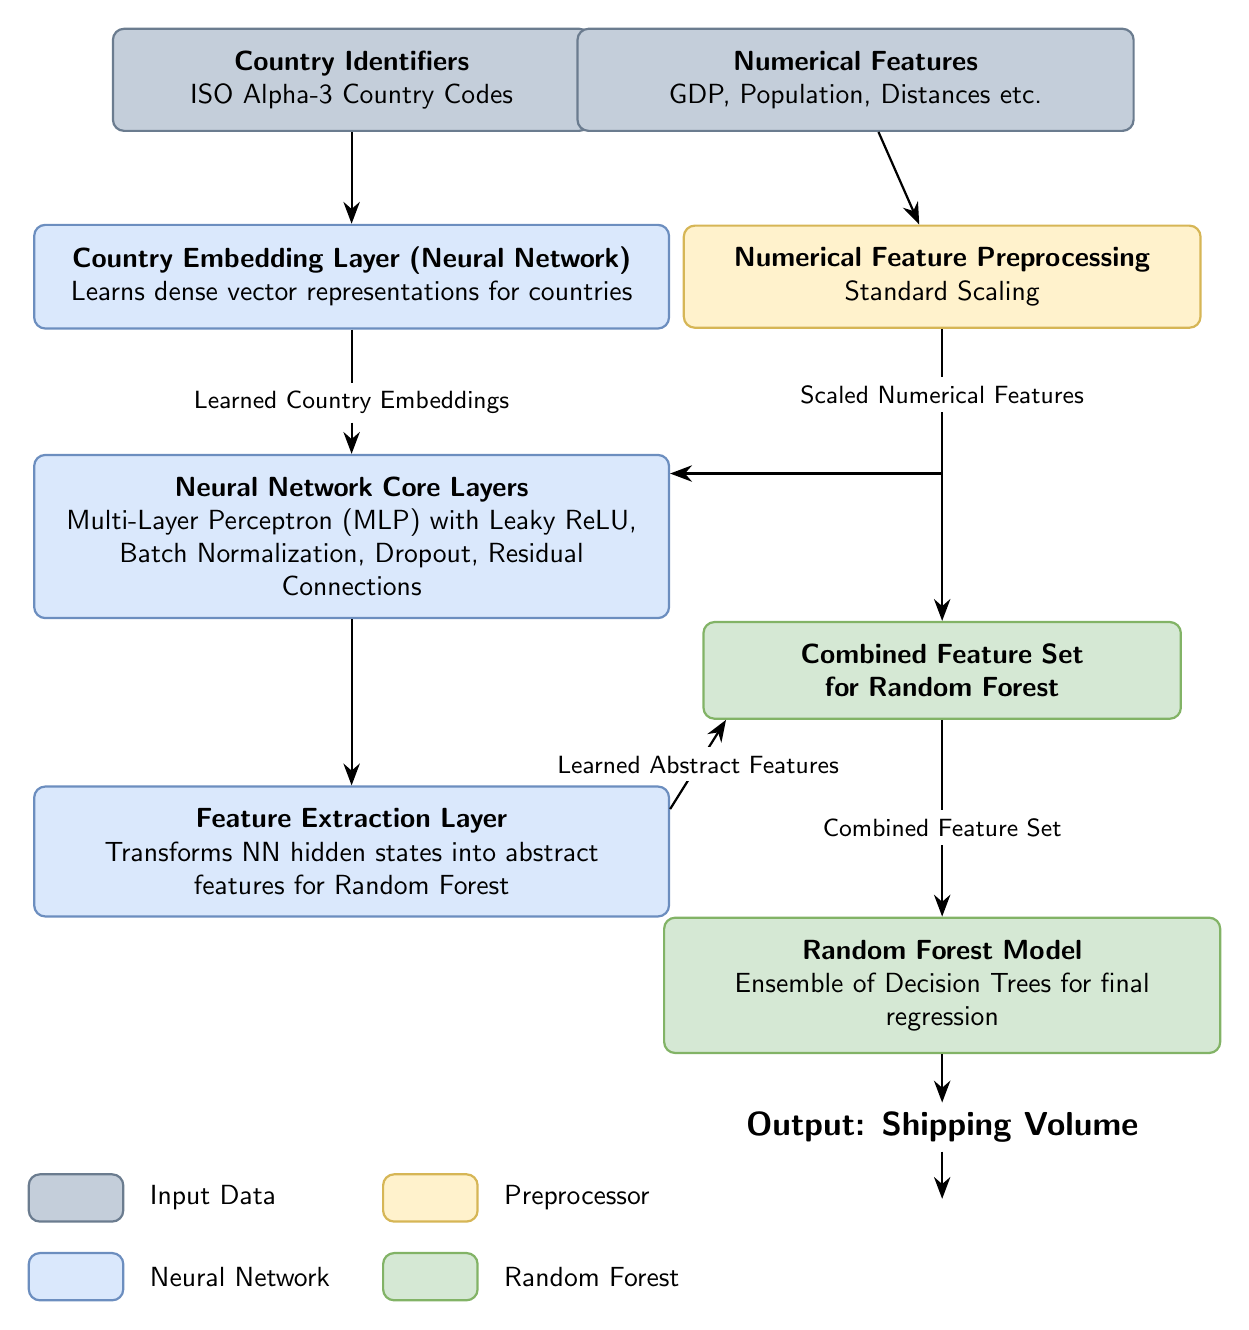
\begin{tikzpicture}[
    font=\sffamily,
    >={Stealth[scale=1.2]},
    box/.style={
        draw, rounded corners=4pt, align=center, inner sep=8pt,
        line width=0.8pt
    },
    inputBox/.style={box, fill=bgGray, draw=borderGray},
    nnBox/.style={box, fill=bgBlue, draw=borderBlue},
    prepBox/.style={box, fill=bgYellow, draw=borderYellow},
    rfBox/.style={box, fill=bgGreen, draw=borderGreen},
    edgeLabel/.style={fill=white, inner sep=3pt, font=\small\sffamily, align=center}
]

\node[inputBox, text width=5.5cm] (country) at (0, 0) {\textbf{Country Identifiers}\\ISO Alpha-3 Country Codes};
\node[inputBox, text width=6.5cm] (num) at (6.4, 0) {\textbf{Numerical Features}\\GDP, Population, Distances etc.};

\node[nnBox, text width=7.5cm] (emb) at (0, -2.5) {\textbf{Country Embedding Layer (Neural Network)}\\Learns dense vector representations for countries};
\node[prepBox, text width=6cm] (prep) at (7.5, -2.5) {\textbf{Numerical Feature Preprocessing}\\Standard Scaling};

\node[nnBox, text width=7.5cm] (core) at (0, -5.8) {\textbf{Neural Network Core Layers}\\Multi-Layer Perceptron (MLP) with Leaky ReLU,\\Batch Normalization, Dropout, Residual\\Connections};

\node[rfBox, text width=5.5cm] (comb) at (7.5, -7.5) {\textbf{Combined Feature Set}\\\textbf{for Random Forest}};

\node[nnBox, text width=7.5cm] (ext) at (0, -9.8) {\textbf{Feature Extraction Layer}\\Transforms NN hidden states into abstract\\features for Random Forest};

\node[rfBox, text width=6.5cm] (rf) at (7.5, -11.5) {\textbf{Random Forest Model}\\Ensemble of Decision Trees for final\\regression};

\node[font=\bfseries\large] (out) at (7.5, -13.3) {Output: Shipping Volume};

\draw[->, thick] (country) -- (emb);
\draw[->, thick] (num) -- (prep);

\node[edgeLabel] (embText) at (0, -4.1) {Learned Country Embeddings};
\draw[thick] (emb.south) -- (embText.north);
\draw[->, thick] (embText.south) -- (core.north);

\node[edgeLabel] (scaledText) at (7.5, -4.0) {Scaled Numerical Features};
\draw[thick] (prep.south) -- (scaledText.north);
\draw[thick] (scaledText.south) -- (7.5, -5.0) coordinate (split);
\draw[->, thick] (split) -- (core.east |- split);
\draw[->, thick] (split) -- (comb.north);

\draw[->, thick] (core.south) -- (ext.north);

\draw[->, thick] ([yshift=-0.3cm]ext.north east) -- ([xshift=0.3cm]comb.south west) node[midway, edgeLabel] {Learned Abstract Features};

\node[edgeLabel] (combText) at (7.5, -9.5) {Combined Feature Set};
\draw[thick] (comb.south) -- (combText.north);
\draw[->, thick] (combText.south) -- (rf.north);

\draw[->, thick] (rf.south) -- (out.north);
\draw[->, thick] (out.south) -- ++(0, -0.6);


\begin{scope}[shift={(-3.5, -14.2)}]
    \node[inputBox, minimum width=1.2cm, minimum height=0.6cm, inner sep=0pt] (leg1) at (0, 0) {};
    \node[right=0.2cm of leg1, font=\normalsize] {Input Data};

    \node[nnBox, minimum width=1.2cm, minimum height=0.6cm, inner sep=0pt] (leg3) at (0, -1) {};
    \node[right=0.2cm of leg3, font=\normalsize] {Neural Network};

    \node[prepBox, minimum width=1.2cm, minimum height=0.6cm, inner sep=0pt] (leg2) at (4.5, 0) {};
    \node[right=0.2cm of leg2, font=\normalsize] {Preprocessor};

    \node[rfBox, minimum width=1.2cm, minimum height=0.6cm, inner sep=0pt] (leg4) at (4.5, -1) {};
    \node[right=0.2cm of leg4, font=\normalsize] {Random Forest};
\end{scope}

\end{tikzpicture}
\end{document}